\documentclass[parskip]{scrartcl}
\usepackage[utf8]{inputenc}

\usepackage[spanish]{babel}
\selectlanguage{spanish}

\usepackage{amsmath}
\usepackage{tikz}
\usepackage{circuitikz}
\usepackage{listings}

\usepackage{pgfplots}

\usepackage{courier}
\usepackage{caption}

\title{Modelo del Filtro RC Low Pass y Análisis Mediante la Transformada de Laplace}
\author{Adrián Barreal}

\newcommand{\laplace}[1]{\mathcal{L}\left\{\,#1\,\right\}}

\lstset{
  basicstyle=\footnotesize\ttfamily,
  numberstyle=\tiny,
  numbersep=5pt,
  tabsize=2,
  extendedchars=true,
  breaklines=true,
  keywordstyle=\color{red},
  frame=b,         
  stringstyle=\color{white}\ttfamily,
  showspaces=false,
  showtabs=false,
  xleftmargin=17pt,
  framexleftmargin=17pt,
  framexrightmargin=5pt,
  framexbottommargin=4pt,
  showstringspaces=false
}

\begin{document}


\maketitle

\begin{abstract}
\noindent En este artículo se ejemplifica el procedimiento necesario para analizar un sistema eléctrico mediante la transformada de Laplace.
Concretamente, se estudia el filtro RC low pass: se construye un modelo diferencial recurriendo a los principios básicos del análisis de circuitos, y se procede luego a obtener la función de transferencia del sistema. La efectividad del modelo se evalúa luego con un caso experimental concreto, obteniendo muy buenos resultados. Para el desarrollo del experimento se utiliza la plataforma Arduino.
\end{abstract}

\tableofcontents

\newpage
\section{Filtro RC Low Pass}

Supongamos que tenemos un componente como el de la figura \ref{fig:rc}. Si imponemos una señal de tensión $v_{\mathrm{in}}(t)$ entre las terminales de entrada, podremos notar que entre las terminales de salida se mide una señal modificada $v_{\mathrm{out}}(t)$.

% Algún ejemplo...

\begin{figure}[h]
\centering
\begin{circuitikz}[american voltages]

\draw (0, 2)
to [short, o-] (2, 2)
to [R=$R$] (4, 2)
to [C=$C$] (4, 0)
to [short, -o] (0, 0);

\draw (4, 2)
to [short, -o] (7, 2);

\draw (4, 0)
to [short, -o] (7, 0);

\draw (0, 2)
to [open,v=$v_\mathrm{in}(t)$] (0, 0);

\draw (7, 2)
to [open,v=$v_\mathrm{out}(t)$] (7, 0);

\end{circuitikz}
\caption{Componente RC.}
\label{fig:rc}
\end{figure}

\subsection{Análisis del Circuito}

Podemos calcular $v_{\mathrm{out}}(t)$ en función de $v_{\mathrm{in}}(t)$ analizando el efecto que tiene el circuito sobre las componentes en frecuencia de la señal de entrada. Para ello, escribimos primero la ecuación diferencial que describe la operatoria del sistema. Sabemos que en todo instante de tiempo $t$, el total entre la caída de tensión $v_R(t)$ a través de la resistencia y la tensión generada entre las placas del capacitor $v_C(t)$ debe ser igual a la tensión $v_{\mathrm{in}}(t)$ impuesta entre las terminales de entrada:
%
\begin{equation}\label{eq:rcbalance}
v_{\mathrm{in}}(t) \;=\; v_R(t) + v_C(t) \,.
\end{equation}

\begin{figure}[t]
\centering
\begin{circuitikz}[american voltages]

\draw (0, 2)
to [short,i=$i(t)$] (2, 2)
to [R=$R$] (4, 2)
to [C=$C$] (4, 0)
to [short] (0, 0);

\draw (4, 2)
to [short, -o] (7, 2);

\draw (4, 0)
to [short, -o] (7, 0);

\draw (7, 2)
to [open,v=$v_\mathrm{out}(t)$] (7, 0);

\draw (0, 0)
to [vsourcesin,l^=$v_\mathrm{in}(t)$] (0, 2);

\end{circuitikz}
\caption{Circuito RC con salida.}
\label{fig:closedrc}
\end{figure}

Si se cierra el circuito entre las terminales de entrada como en la figura \ref{fig:closedrc}, sabemos que circulará una corriente $i(t)$ tal que $v_R(t)$ sea simplemente $R\,i(t)$. Por otro lado, asumiendo que está inicialmente descargado, sabemos que la carga total $q(t)$ acumulada en el capacitor en un instante $t$ será la acumulación de la carga que circuló por el circuito desde el instante $0$ hasta el instante $t$:
%
$$ q(t) \;=\; \int_0^{\,t} i(\tau)\,d\tau \,. $$

Sabemos también que la capacitancia nos indica la carga que acumula el capacitor por unidad de voltaje entre sus placas, por lo que $v_C(t) = q(t)/C$ y por lo tanto, podemos escribir \eqref{eq:rcbalance} como
%
$$ v_{\mathrm{in}}(t) \;=\; R\,i(t) \;+\; \frac{1}{C} \int_0^{\,t} i(\tau)\,d\tau \,. $$

Asumiendo que la señal de entrada tiene transformada de Laplace, pasamos al dominio de la frecuencia aplicando el operador a cada lado de la igualdad:
%
\begin{equation} \label{eq:rclaplace1}
\laplace{v_{\mathrm{in}}(t)} \;=\;
\left(\, R + \frac{1}{sC} \,\right)\laplace{i(t)}
,\quad \mathrm{con}\;\,\laplace{f(t)} \equiv \int_0^\infty f(t)\,e^{-st}\,dt \,.
\end{equation}

Por otro lado, podemos escrbir también
%
$$ \laplace{v_C(t)} 
\;=\; \frac{1}{C}\;\laplace{\int_0^{\,t} i(\tau)\,d\tau}
\;=\; \frac{1}{sC}\,\laplace{i(t)} \,.$$

Reemplazando $\laplace{i(t)}$ en \eqref{eq:rclaplace1} obtenemos finalmente
%
\begin{equation}\label{eq:rctransfer}
H(s)
\;=\; \frac{\laplace{v_C(t)}}{\laplace{v_\mathrm{in}(t)}} 
\;=\; \frac{1}{1 + sRC}\,.
\end{equation}

Considerando que $v_C(t)$ es efectivamente $v_{\mathrm{out}}(t)$, la expresión \eqref{eq:rctransfer} define la función de transferencia del sistema,
que relaciona la salida con la entrada en el dominio de la frecuencia.

Podemos determinar cómo el circuito afecta la amplitud en cada frecuencia evaluando la ganancia del sistema. Evaluamos la función de transferencia en la frecuencia angular compleja $j\omega$, donde $j$ es la unidad imaginaria.
%
$$ \lvert\,H(j \omega)\,\rvert = \frac{1}{\sqrt{1 + (\omega RC)^2}}\,, $$

La ganancia en función de la frecuencia angular se muestra gráficamente en la figura \ref{fig:rcgain}, para algún $RC$ fijo. Podemos ver que, en esta configuración, a medida que la frecuencia angular aumenta la amplitud de la componente harmónica disminuye; es decir, las frecuencias más altas se verán atenuadas por el efecto del circuito.

\begin{figure}[t]
\centering
\begin{tikzpicture}
  \begin{axis}[
      ymin = 0,
      ymax = 1,
      axis y line=center,
      axis x line=center,
      xlabel=$\omega$,
      ylabel={$\quad \lvert\,H(j \omega)\,\rvert$},
      ytick={0.25, 0.5, 0.75},
      extra y ticks={1},
      yticklabels={},
      extra y tick style={yticklabel=\pgfmathprintnumber{\tick}},
      xticklabels={}
    ] 
    \addplot[
      smooth,
      mark=none,
      samples=40,
      domain=-10:10
    ] {1/sqrt(1 + x^2)}; 
  \end{axis}
\end{tikzpicture}
\caption{Ganancia del sistema en función de la frecuencia angular $\omega$.}
\label{fig:rcgain}
\end{figure}

\section{Verificación Experimental}

\subsection{Caso Propuesto}

En un instante de tiempo $t = 0$, se genera un pulso de tensión de amplitud $V$ y duración $T$ como se muestra en la figura \ref{fig:pulse}. La señal en cuestión puede representarse matemáticamente mediante la función escalón de Heaviside $\mu$:
%
$$ v_\mathrm{in}(t) = V\,\left[\, \mu(t) - \mu(t - T) \,\right] $$

La transformada de Laplace de $v_\mathrm{in}(t)$ existe y está dada por
%
\begin{equation}\label{eq:pulsetransform}
\laplace{v_\mathrm{in}(t)} \;=\; \frac{V}{s}\,\left(\,1 - e^{-sT}\,\right)
\end{equation}

Del producto entre \eqref{eq:pulsetransform} y la función de transferencia \eqref{eq:rctransfer} resulta la transformada de Laplace de la respuesta del circuito ante el pulso de entrada:
%
$$
\laplace{v_\mathrm{out}(t)} \;=\; \frac{V}{s + RC s^2}\,\left(\,1 - e^{-sT}\,\right)
$$

Determinando la transformada inversa encontramos entonces la respuesta del sistema en el dominio del tiempo, ante el pulso de entrada $v_\mathrm{in}(t)$:
%
\begin{equation}\label{eq:pulseout}
v_\mathrm{out}(t) \;=\; V \left[\; \mu(t - T)\,\left( e^\frac{T-t}{RC} - 1 \right) - e^\frac{-t}{RC} + 1 \;\right], \quad t \geq 0
\end{equation}

\begin{figure}[t]
\centering
\begin{tikzpicture}
  \begin{axis}[
    axis lines = middle,
    height=4cm,
    width=10cm,
    axis lines*=center,
    ytick={},
    yticklabels={},
    extra y ticks={1},
    extra y tick labels={$V$},
    ymax=1.5,
    xmax=7.5,
    ylabel={$v_\mathrm{in}(t)$},
    ylabel near ticks,
    xlabel={$t$},
    xlabel near ticks,
    xtick={},
    xticklabels={},
    extra x ticks={1},
    extra x tick labels={$T$},
    every axis x label/.style=
      {at={(current axis.right of origin)},anchor=north west},
    ylabel style={rotate=-90}
  ]
  \addplot+[black,mark=none,const plot] 
    coordinates {(0,0) (0,1) (1,1) (1,0) (7,0)};
\end{axis}
\end{tikzpicture}
\caption{Pulso de tensión de amplitud $V$ y duración $T$.}
\label{fig:pulse}
\end{figure}

Concretamente, una resistencia $R = 95\,\mathrm{k\Omega}$, en conjunto con una capacitancia $C = 9.4\,\mathrm{\mu F}$ produce un factor $RC = 0.893\,\mathrm{seg}$. Con dicho factor, la respuesta del sistema ante un pulso de amplitud $V = 5\,\mathrm{Volt}$ y duración $T = 0.5\,\mathrm{seg}$ será similar a la que se muestra en la figura \ref{fig:rcresponse}. Se puede ver como el filtro suaviza la señal debido a la eliminación de las altas frecuencias. Procederemos ahora a verificar el hecho mediante un experimento concreto.

\begin{figure}[t]
\centering
\begin{tikzpicture}
  \begin{axis}[
      height=4cm,
      width=10.5cm,
      ymin = 0,
      ymax = 2.5,
      axis y line=left,
      axis x line=center,
      xlabel=$t$,
      ylabel={$v_\mathrm{out}(t)$},
      extra y tick style={yticklabel=\pgfmathprintnumber{\tick}},
      ylabel style={rotate=-90},
      xtick={},
      xticklabels={},
      extra x ticks={0.5},
      extra x tick labels={$T = 0.5\,\mathrm{seg}$},
    ] 
    \addplot[
      smooth, mark=none, samples=40, domain=0:0.5
    ] {5*(1 - exp(-x/0.893))};
    \addplot[
      smooth, mark=none, samples=40, domain=0.5:4
    ] {5*((exp((0.5 - x)/0.893) - 1) + 1 - exp(-x/0.893)))}; 
  \end{axis}
\end{tikzpicture}
\caption{Respuesta ante un pulso con $V = 5\,\mathrm{Volt}$, $T = 0.5\,\mathrm{mseg}$ 
         y $RC = 0.893\,\mathrm{mseg}$.}
\label{fig:rcresponse}
\end{figure}

\newpage
\subsection{Ejecución del Experimento}

\subsubsection{Esquema Experimental}

En la figura \ref{fig:rcpic} se muestra una foto del esquema experimental utilizado para el desarrollo del experimento. El pulso de tensión se genera entre los pines 13 y GND de Arduino, mediante la función digitalWrite. Entre los rieles positivo y negativo hay colocada una resistencia de aproximadamente $95\,\mathrm{k\Omega}$, en serie con dos capacitores paralelos, cada uno con una capacitancia nominal de $4.7 \mu F$. El cable amarillo va desde el punto entre la resistencia y los capacitores hasta el pin analógico A0 de Arduino; la tensión de salida del filtro es la que se genera entre el cable amarillo y masa, y será medida mediante la función analogRead.\\

\begin{figure}[h]
  \centering
  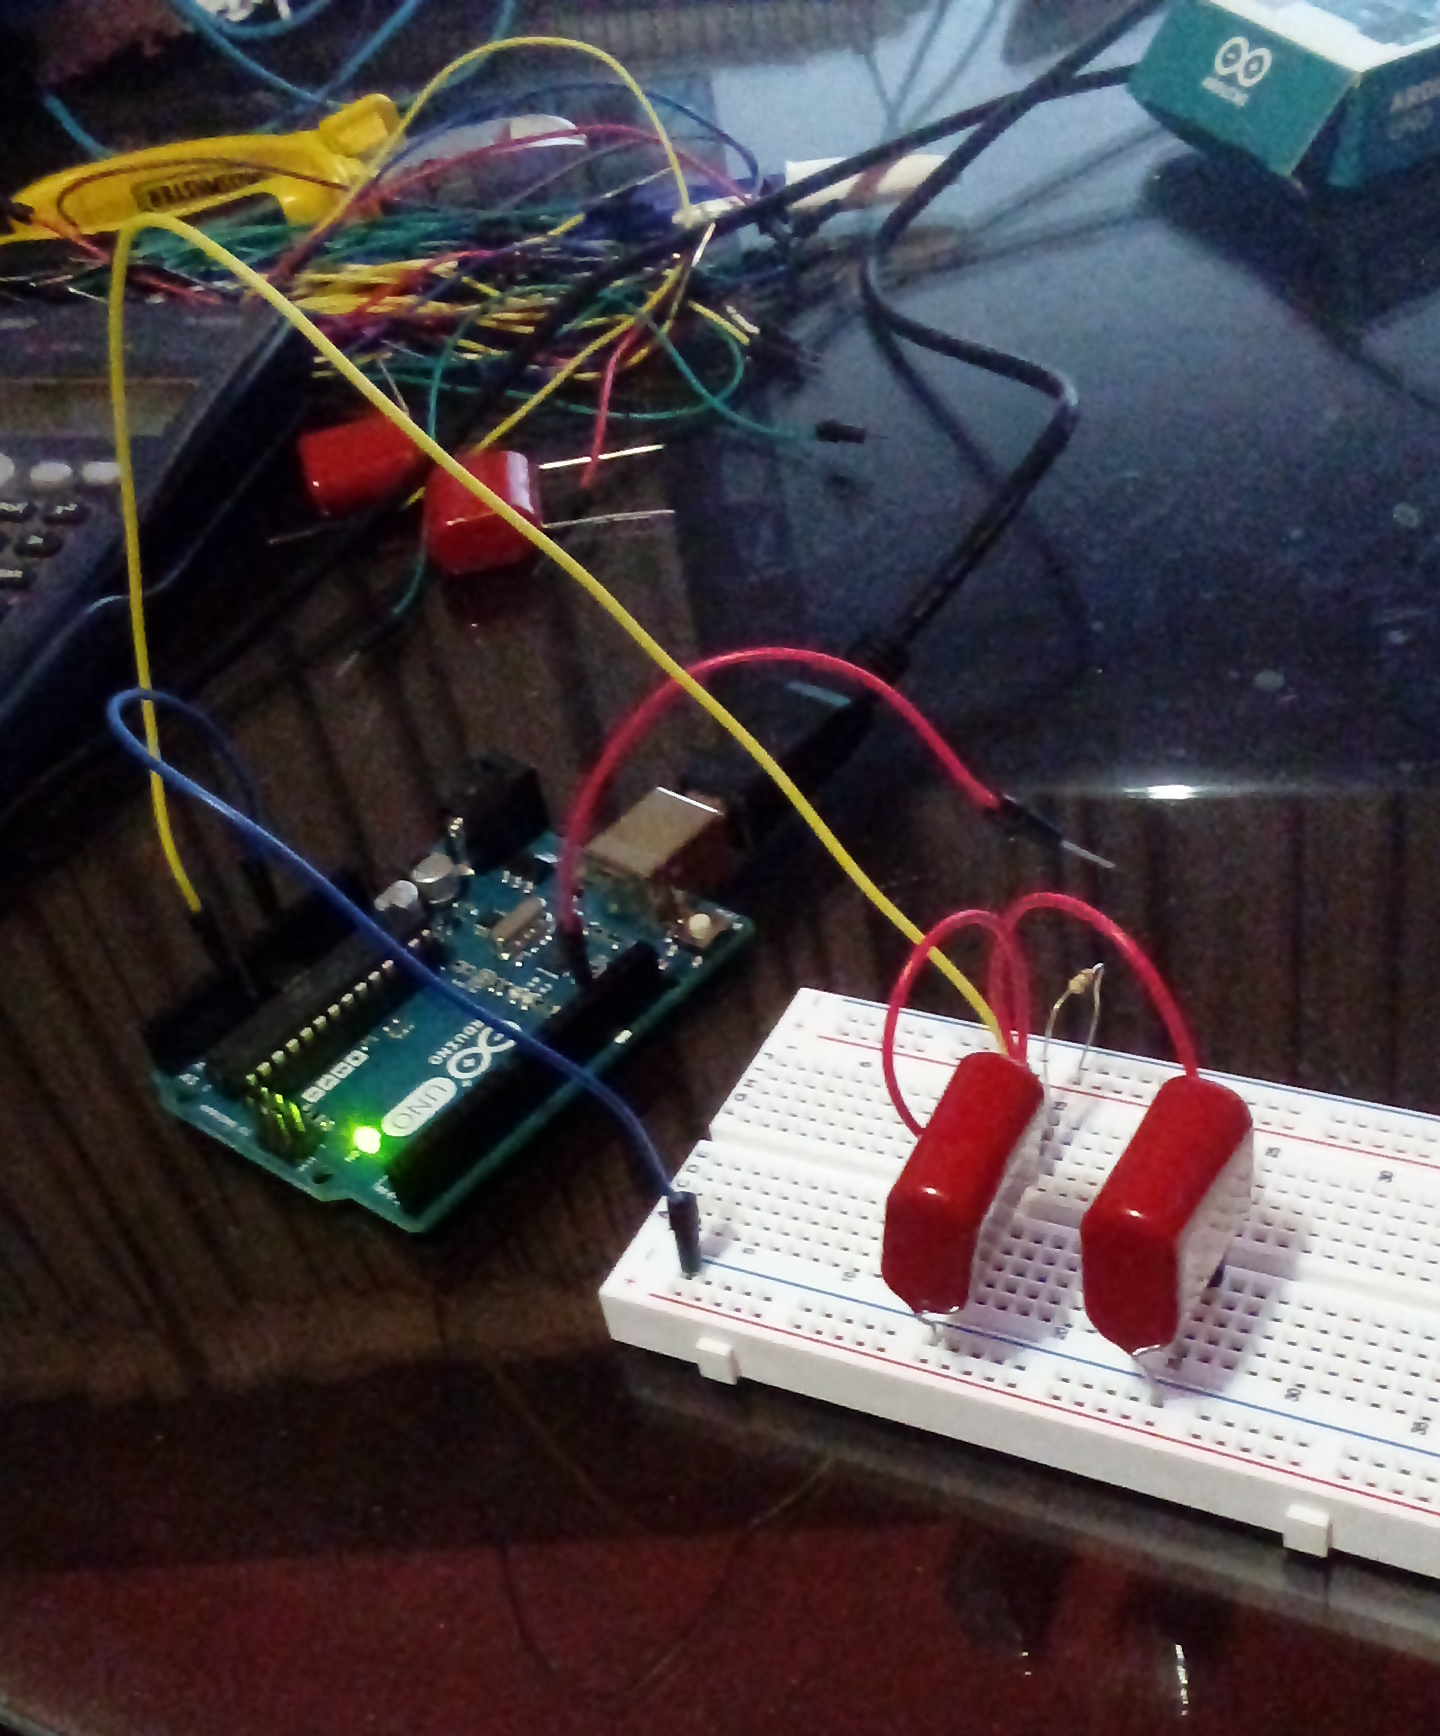
\includegraphics[scale=0.15]{rcpic.png}
  \caption{Foto del esquema experimental; aquí el circuito está todavía abierto.}
  \label{fig:rcpic}
\end{figure}

\subsubsection{Sketch de Arduino}

En la figura \ref{fig:sketch} se muestra el código fuente del sketch utilizado en el experimento. Se toman muestras del pin analógico de entrada cada $50\,\mathrm{mseg}$; las muestras son almacenadas en un arreglo para ser luego emitidas por el puerto serie.

\begin{figure}
\begin{lstlisting}[frame=single]

const int PIN_OUT = 13;
const int PIN_IN = A0;

const int SAMPLE_COUNT = 256;

int time[SAMPLE_COUNT];
int volt[SAMPLE_COUNT];

void measureFor(int duration, int sampling_period, int t0, int i) {
  for (int t = t0; t < t0 + duration; t += sampling_period, i++) {
    time[i] = t;
    volt[i] = analogRead(PIN_IN);
    delay(sampling_period);
  }
}

void setup() {
  Serial.begin(9600);
  pinMode(PIN_OUT, OUTPUT);
}

void loop() {
  digitalWrite(PIN_OUT, HIGH);
  measureFor(500, 50, 0, 0);
  digitalWrite(PIN_OUT, LOW);
  measureFor(5000, 50, 500, 10);
  delay(4500);
  
  for (int i = 0; i < SAMPLE_COUNT; i++) {
    Serial.print("(");
    Serial.print(time[i]);
    Serial.print(",");
    Serial.print(volt[i] * (5.0/1023.0));
    Serial.println(")");
  }
}

\end{lstlisting}
\caption{Código fuente del sketch de Arduino.}
\label{fig:sketch}
\end{figure}

\subsection{Resultados Experimentales}

En la figura \ref{fig:rcresponseempiric} se muestra un gráfico con algunos de los valores medidos durante la ejecución del experimento. En él se pueden observar los patrones de crecimiento y decaimiento predichos por la solución analítica.

Para evitar saturar el gráfico, en la curva de crecimiento se muestran valores cada $100\,\mathrm{mseg}$, y en el decaimiento se muestran valores cada $200\,\mathrm{mseg}$, a pesar de que las muestras se tomaron cada $50\,\mathrm{mseg}$; el conjunto completo de todas las muestras adquiridas se puede encontrar en la página siguiente.

\begin{figure}[h!]
\centering
\begin{tikzpicture}
  \begin{axis}[
      height=4cm,
      width=10.5cm,
      ymin = 0,
      ymax = 2.5,
      axis y line=left,
      axis x line=center,
      xlabel=$t\;(\mathrm{msec})$,
      ylabel={$v_\mathrm{out}(t)$},
      extra y tick style={yticklabel=\pgfmathprintnumber{\tick}},
      ylabel style={rotate=-90},
      every axis x label/.style={
        at={(ticklabel* cs:1.05)},
        anchor=west,
      }
    ] 
    \addplot[black,mark=*] coordinates {
      (0,0.00)
      (100,0.50)
      (200,0.95)
      (300,1.36)
      (400,1.73)
      (500,2.06)
      (700,1.66)
      (900,1.34)
      (1100,1.08)
      (1300,0.87)
      (1500,0.70)
      (1700,0.56)
      (1900,0.45)
      (2100,0.37)
      (2300,0.29)
      (2500,0.23)
      (2700,0.19)
      (2900,0.15)
      (3100,0.12)
      (3300,0.09)
      (3500,0.07)
      (3700,0.06)
      (4000,0.04)
    };
  \end{axis}
\end{tikzpicture}
\caption{Respuesta de un filtro RC ante un pulso; resultados experimentales.}
\label{fig:rcresponseempiric}
\end{figure}

Para evaluar la fidelidad de la predicción en forma cuantitativa, evaluamos la expresión \eqref{eq:pulseout} de la respuesta del sistema con $RC = 0.893$ milisegundos. Este valor de $RC$ fue calculado en base a las capacitancias nominales y a la resistencia medida con multímetro. En $t = 0.5\,\mathrm{mseg}$, se estima una tensión de salida de $2.14\,\mathrm{Volt}$, muy cercana a la que se mide experimentalmente ($2.06\,\mathrm{Volt}$), siendo el error porcentual inferior a $4$\%. Evaluando sobre la curva de decaimiento, en $t = 1\,\mathrm{mseg}$, se obtiene un valor analítico para la salida de $1.22\,\mathrm{Volt}$. El error porcentual con respecto al valor medido es cercano a $2$\%, siendo este último de $1.20\,\mathrm{Volt}$.

Considerando que no se tomó ningún tipo de medida para reducir el margen de error, podemos concluir que el modelo aplicado es muy efectivo para predecir el comportamiento del circuito RC.

\section{Conclusiones}

Podemos concluir que los métodos analíticos son herramientas muy potentes para predecir el comportamiento de los sistemas eléctricos. La función de transferencia provee un mecanismo muy eficiente para encapsular el comportamiento de un sistema complejo en una expresión simple, sin afectar de ninguna forma la precisión del modelo físico subyacente, el cuál en este caso demostró ser muy bueno. En adición, hay que mencionar la facilidad que provee la plataforma Arduino para la ejecución de experimentos físicos.

\newpage
\begin{verbatim}
TIME VOLTAGE
msec volt
   0 0.00    1500 0.70    3000 0.13    4500 0.02
  50 0.25    1550 0.66    3050 0.13    4550 0.02
 100 0.50    1600 0.63    3100 0.12    4600 0.01
 150 0.73    1650 0.60    3150 0.11    4650 0.01
 200 0.95    1700 0.56    3200 0.10    4700 0.01
 250 1.16    1750 0.54    3250 0.10    4750 0.01
 300 1.36    1800 0.50    3300 0.09    4800 0.01
 350 1.55    1850 0.48    3350 0.09    4850 0.01
 400 1.73    1900 0.45    3400 0.09    4900 0.01
 450 1.90    1950 0.43    3450 0.08    4950 0.01
 500 2.06    2000 0.41    3500 0.07    5000 0.00
 550 1.95    2050 0.38    3550 0.07    5050 0.00
 600 1.85    2100 0.37    3600 0.07    5100 0.00
 650 1.75    2150 0.34    3650 0.06    5150 0.00
 700 1.66    2200 0.32    3700 0.06    5200 0.01
 750 1.57    2250 0.31    3750 0.05    5250 0.00
 800 1.49    2300 0.29    3800 0.05    5300 0.00
 850 1.41    2350 0.27    3850 0.05    5350 0.00
 900 1.34    2400 0.26    3900 0.04    5400 0.00
 950 1.27    2450 0.24    3950 0.04    5450 0.00
1000 1.20    2500 0.23    4000 0.04    
1050 1.14    2550 0.22    4050 0.03    
1100 1.08    2600 0.21    4100 0.03    
1150 1.03    2650 0.20    4150 0.03    
1200 0.97    2700 0.19    4200 0.03    
1250 0.92    2750 0.18    4250 0.02    
1300 0.87    2800 0.17    4300 0.03    
1350 0.82    2850 0.16    4350 0.02    
1400 0.78    2900 0.15    4400 0.02    
1450 0.74    2950 0.14    4450 0.02    

\end{verbatim}

\end{document}
